\documentclass[../SWD_disp.tex]{subfiles}

\begin{document}
\section{Strategy og Template Method Pattern}

\subsection*{Hvad er et Design Pattern?}
Ideen med et design pattern er, at det kan beskrives som et problem, der forekommer igen og igen, og beskriver kernen i dette problem. Det der gør dette til et pattern er, at problemet og løsningen kan genbruges uden at man gør det samme. Ved anvendelse af et design pattern, skal der altid tilbasses det specifikke problem, man sidder med. Overordnet er det en form for skabelon til løsning af et problem. Dog kan denne ikke være gældende for alle tilfælde. Dette er fordi, det skal modificeres i forhold til problemet man sidder med.
\\

I løbet af kurset er GoF design patterns (Gang of Four) blevet gennemgået. Der er 23 patterns opdelt i 3 grupper. Disse 3 grupper definerer følgende

\begin{itemize}
    \item \textbf{Creational Patterns:} Fortæller hvordan objekter oprettet på en fornuftig måde
    \item \textbf{Structural Patterns:} Fortæller hvordan koden skal struktureres, således at den er fleksibel eller reusable osv. (Dette svare til et klassediagram)
    \item \textbf{Behaviour:} Fortæller om adfærd og hvordan koden skal opføre sig for, at blive fleksibel eller reusable osv. (Dette svare til et sekvensdiagram)
\end{itemize}
\subsection{SKRIV OM ET PNG PATTERN}
\subsection*{GoF Strategy Pattern}
Et strategy pattern definerer følgende punkter

\begin{itemize}
    \item Definerer en sæt af algoritmer
    \item Indkapsler hver algoritme i dens egen klasse
    \item Opretter en udskiftelig familie af algoritmer, alt efter hvad der er behov for. Dette udvælges under run-time.
    \item Tilhører behavioral pattern (specificerer hvordan komminukationen mellem klasser skal foregå)
\end{itemize}

Figur~\ref{fig:strategy_pattern} viser et eksempel på et Strategy Pattern

\begin{figure}[H]
    \centering
    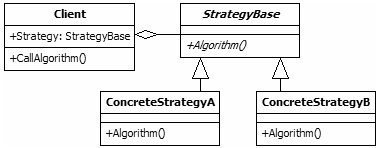
\includegraphics{strategy_pattern.PNG}
    \caption{Strategy Pattern}
    \label{fig:strategy_pattern}
\end{figure}

\textbf{Client:} Denne klasse er brugeren af den udskiftelige algoritme. Dens egenskab er, at holde på en af strategy klasserne. Denne egenskab vil blive sat eller ændret ved run-time.

\textbf{StrategyBase:} Abstrakt klasse, og base klasse for alle klasser, der anvender en algoritme. Dette eksempel har kun 1 modul. Denne klasse kan blive implementeret, som et interface, hvis ikke det har nogle funktioner for dens nedarvede klasser.
\\

\textbf{ConcreteStrategyA/B:} Nedarver fra baseklassen. Hver strategy udgør en forskellig algoritme, der bliver brugt af clienten.

\subsection*{Template Method Pattern}
Template Method Pattern definerer skellettet af en algoritme ud fra en operation. Dette gøres ved, at udsætte steps til clientens subklasser.

\begin{figure}[H]
    \centering
    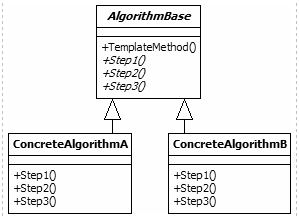
\includegraphics{template_method_pattern.PNG}
    \caption{Template Method Pattern}
    \label{fig:template_method_pattern}
\end{figure}

\textbf{AlgorithmBase:} Abstrakt klasser der er base klassen for alle concrete versioner af algoritmen. Klassen definerer abstrakte metoder, for hver af de steps, der kan blive justeret af subklasserne. Den består også af en enkelt metode, der kontrollerer algoritmen og kalde de individuelle steps.
\\

\textbf{ConcreteAlgorithmA/B:} Nedarver fra base klassen. Disse algoritmer \textbf{overrider} abstrakte sted metoder, for at give reele implementeringer. Dog overrider den ikke TemplateMethod().
\\

Ved bruge af Template Method Pattern, holder den abstrakte klasse en generel algoritme i en metode. Denne metode lader subklasser de konkrete skrift i denne algoritme. På denne måde, kan den generelle algoritme anvendes til mange situationer. Detfor skal der i dette pattern være en abstrakt klasser, som template for de nedarvede klasser, samt i den klasser der har algoritmens steps, således at subklasserne kan override dem.

\subsection*{Sammenligning. Hvornår og hvorfor de anvendes.}
Template Method Pattern og Strategy Pattern gør stort set det samme.
\\

Strategy Pattern når adfærden varierer ved runtime, og det er meget let at tilføje nye adfærd.
\\

Template Method Pattern bruger nedarvning og adfærden bliver ændret ved compile time. Nedarvede klasser består af dele af algoritmen.
\\

Til test vil Strategy Pattern være bedst pga. interface. Hvis man har et lille system, vil Template Method være fint, da man ikke behøver at skrive meget kode dertil.
\end{document}
